\documentclass{report}
\usepackage[utf8]{inputenc}

\usepackage[italian]{babel}
\usepackage{graphicx}
\usepackage{float}
\usepackage{hyperref}
\usepackage[italian]{cleveref}

\title{OOP-FARGOAL}
\author{
    Bulgarelli Marco, marco.bulgarelli6@studio.unibo.it \and 
    Ravaioli Alessandro, alessandro.ravaioli8@studio.unibo.it \and
    Tassinari Sabrina, sabrina.tassinari@studio.unibo.it \and
    Tramonti Daniele, daniele.tramonti2@studio.unibo.it 
}
\date{15 febbraio 2025}

\begin{document}
\maketitle

\tableofcontents

\chapter{Analisi}

\section{Descrizione e requisiti}

Il software mira alla costruzione di un videogioco ispirato a “Sword of Fargoal” \footnote{
    Il videogioco è stato realizzato da Epyx nel 1982 per VIC-20, l'anno dopo è stato rilasciato per Commodore 64.
}. 
%
Quest’ultimo è un “Dungeon Crawler Arcade”, ovvero basato sull’esplorazione di un labirinto a più piani, con lo scopo di riportare in superficie la Spada di Fargoal attraversando innumerevoli pericoli. 
%
La nostra versione cercherà di essere il più fedele possibile al gioco originale.

\subsection{Requisiti funzionali}
\begin{itemize}
    \item Il giocatore si muoverà all’interno di una grande stanza che corrisponde ad un piano del Dungeon. La generazione di ogni piano (e dei suoi contenuti) dovrà essere casuale.
    \item Il piano è caratterizzato dalla presenza di mostri. Questi possono apparire in luoghi specifici o in punti casuali, aumentando gradualmente con il passare del tempo, rendendo l’ambiente sempre più pericoloso.
    \item All’interno del piano saranno presenti due tipologie di oggetti di cui il giocatore potrà usufruire: dei bauli, che possono contenere degli oggetti magici o delle trappole, oppure delle sacche di monete.
    \item Il sistema di progresso del personaggio è legato all’accumulo di esperienza, che contribuisce all’aumentare del suo livello. Questa può essere ottenuta sia combattendo contro i mostri che offrendo donazioni in oro ai templi.
    \item In ogni piano sarà presente almeno un tempio, dove è possibile donare oro per salire di livello, rigenerare punti ferita e, ogni volta che sono state donate 2000 monete, di essere curati completamente. Inoltre, i templi garantiscono temporanea inattaccabilità ed una rigenerazione accelerata.
    \item Una volta recuperata la spada, è necessario riportarla in superficie, ritornando al primo piano e salendo le scale per uscire dal labirinto. La sfida sta nel fatto che, se il giocatore viene attaccato da un mostro, perde la spada, che ritornerà automaticamente nel piano in cui è stata trovata.
\end{itemize}

\subsection{Modello del dominio}

Il labirinto (\textit{dungeon}) è formato da più piani (\textit{Floor}). 
%
Per muoversi fra un piano e l’altro si utilizzeranno delle rampe di scale; in uno stesso piano saranno presenti più rampe per risalire o per scendere. 
%
Ogni volta che si entra in un nuovo piano, che sia antecedente o successivo, esso verrà generato casualmente. 
%
All’interno di ogni piano saranno presenti vari elementi (in \ref{img:DiagrammaUMLAnalisi} si chiamano \textit{FloorElement}): alcuni hanno la caratteristica di essere interagibili (in \ref{img:DiagrammaUMLAnalisi} \textit{Interactable}), mentre gli altri elementi sono delle entità (\textit{Entity}), che si muovono all’interno del piano. 
%
I primi, che sono fissi nella mappa, sono l’insieme formato dalle ceste (che contengono oggetti magici), le scale (in \ref{img:DiagrammaUMLAnalisi} \textit{Stairs}) e il tempio (in \ref{img:DiagrammaUMLAnalisi} \textit{Temple}) , che è unico all’interno del piano. 
%
Le entità, invece, sono l’insieme dei mostri (in \ref{img:DiagrammaUMLAnalisi} \textit{Monster}) e del giocatore (in \ref{img:DiagrammaUMLAnalisi} \textit{Player}); entrambi si muovono liberamente all’interno del piano e possono entrare in combattimento l’uno con l’altro. 

\begin{figure}
    \centering
    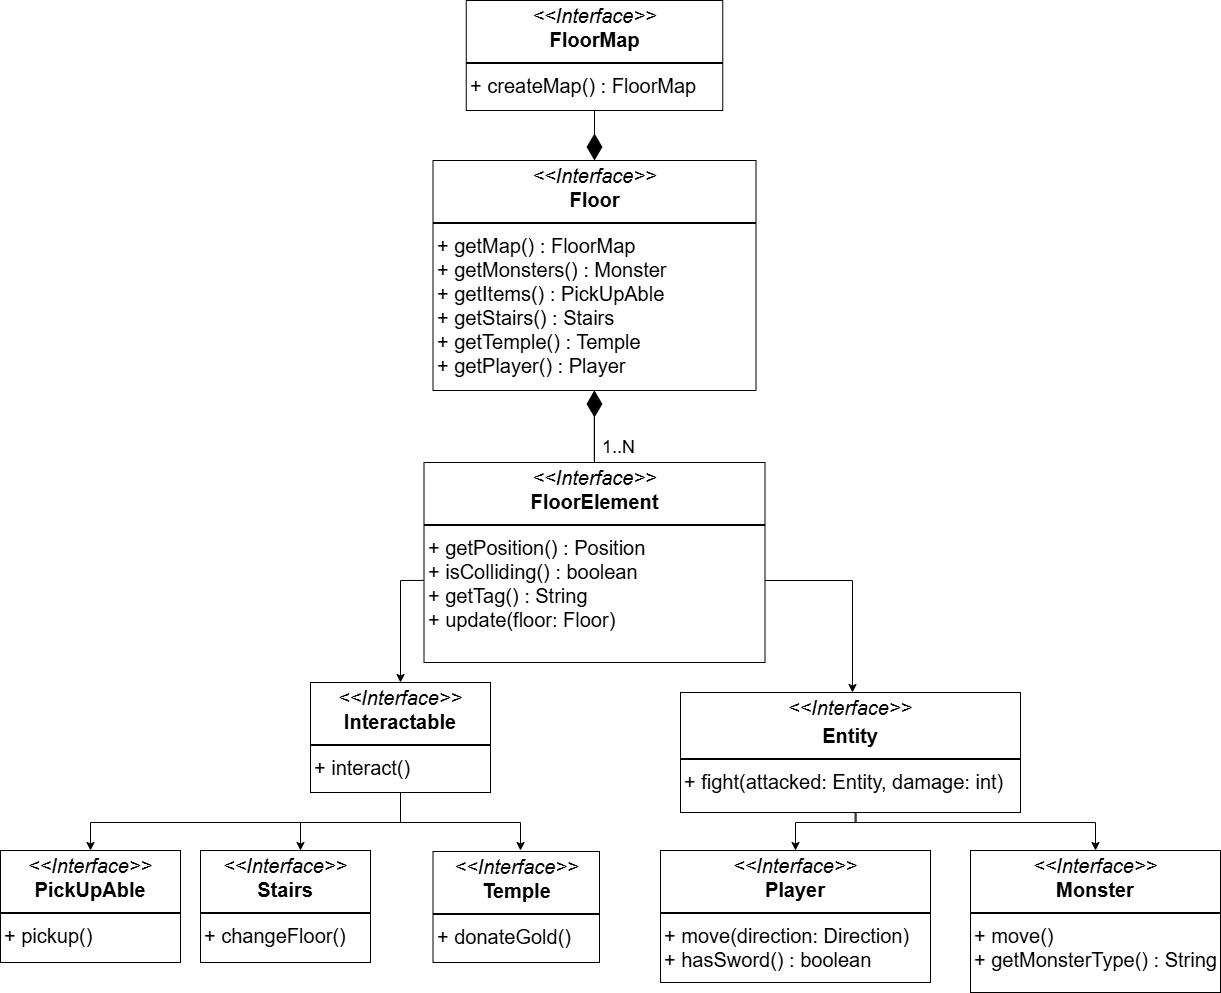
\includegraphics[width=12cm]{DiagrammaAnalisi.drawio.png}
    \caption{Schema UML dell'analisi del problema, con rappresentate le entità principali ed i rapporti fra di loro}
    \label{img:DiagrammaUMLAnalisi}
\end{figure}

\chapter{Design}

\section{Architettura}

L'architettura dell'applicazione segue il pattern architetturale MVC. Il punto di partenza della nostra applicazione è la classe \textit{GameEngine} che inizializza \textit{View, Model} e \textit{Controller}. 
%
La \textit{View} è il punto d'ingresso degli input, la quale li riceve ed in seguito notifica l'\textit{InputController}. Quest'ultimo grazie all' \textbf{InputComponent} riesce ad aggiornare 
%
il \textit{Model}, che nel nostro caso è la \textbf{SceneManager}. Questa è estesa da \textbf{FloorManager}, interfaccia che si occupa di gestire collisioni e gestire ed aggiornare
%
gli elementi attivi nel piano. Infine utilizzando l'interfaccia \textbf{Renderer}, i vari \textit{FloorElement} vengono aggiunti in coda nella \textit{View} in attesa di essere
%
ridisegnati nel seguente \textbf{update()}.
%

\begin{figure}[H]
    \centering{}
    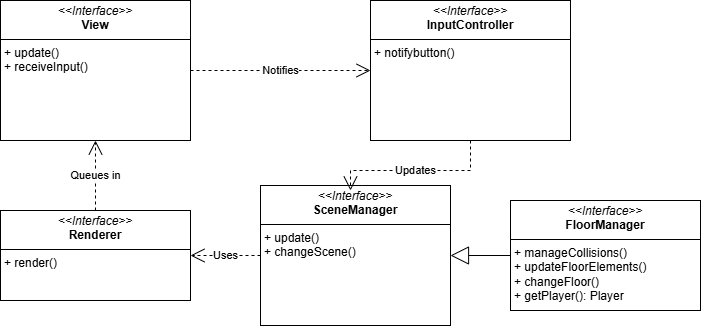
\includegraphics[width=13cm]{MVCProgetto.png}
    \caption{Architettura dell'applicazione (MVC)}
    \label{img:analysis}
\end{figure}

\section{Design dettagliato}

\subsection{Bulgarelli Marco}

\subsubsection{Organizzazione del Player}

\paragraph{Problema} Fornire interfacce che permettano una gestione più efficiente del Player e migliorare la leggibilità del codice.

\paragraph{Soluzione} Suddivisione della gestione del Player in tre classi specifiche, ognuna con un ruolo ben definito:

\begin{itemize}
    \item \textit{Inventory} per la gestione dell'inventario.
    \item \textit{Gold} per la gestione del denaro.
    \item \textit{Health} per la gestione dei punti vita.
\end{itemize}

La classe \textit{PlayerImpl} si compone di due elementi fondamentali per la supervisione delle risorse del giocatore: \textit{Inventory} e \textit{Gold}. \newline
%
\textit{Inventory}, implementato da \textit{InventoryImpl}, gestisce gli oggetti del giocatore, consentendo di aggiungerli, rimuoverli e monitorarne la quantità
%
all’interno dell’inventario. \textit{Gold}, implementato da \textit{GoldImpl}, gestisce invece il numero di monete trasportate dal Player, il limite massimo trasportabile
%
e le donazioni effettuate al tempio. \newline
%
Separare questa logica dalla classe \textit{PlayerImpl} evita ridondanze e migliora la leggibilità del codice. \newline
%
Oltre a queste componenti, \textit{PlayerImpl} include \textit{Health}, la cui implementazione \textit{HealthImpl} si occupa della gestione dei punti vita del giocatore e
%
delle operazioni correlate. Questa classe è stata progettata a livello di entità (\textit{Entity}) per consentirne il riutilizzo anche da parte dei mostri, garantendo maggiore flessibilità. \newline
%
Grazie a questa suddivisione, il codice risulta più leggibile, modulare ed estensibile, facilitando future modifiche e aggiunte senza compromettere la chiarezza della struttura.

\begin{figure}[H]
    \centering
    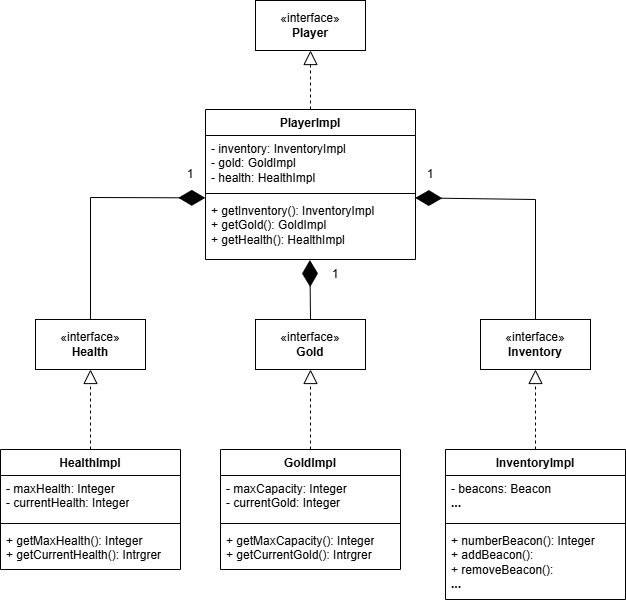
\includegraphics[width=13cm]{PlayerImpl.png}
    \caption{Schema UML delle classi che compongono \textit{PlayerImpl} usate per semplificare l'organizzazione del Player.}
    \label{img:PlayerImpl.png}
\end{figure}

\paragraph{Problema} Gestione dell’input da tastiera, evitando di creare dipendenze tra model e view.

\paragraph{Soluzione} Utilizzo del pattern di progettazione Observer. \newline
%
L’interfaccia \textit{View} è responsabile della ricezione degli input direttamente dal Client. Una volta acquisiti, questi input vengono trasmessi all’interfaccia \textit{InputController}, 
%
che viene implementata da \textit{KeyboardInputController}. 
%
Il ruolo di \textit{InputController} è quello di fungere da intermediario tra \textit{View} e \textit{InputComponent}, garantendo che le azioni del giocatore vengano interpretate correttamente. \newline 
%
Grazie a \textit{InputController}, il sistema è in grado di rilevare quali tasti vengono premuti e in quale momento, traducendo questi comandi in istruzioni comprensibili per il gioco.
%
Una volta ricevute le informazioni da \textit{InputController}, \textit{InputComponent} le elabora e le utilizza per eseguire le azioni richieste dal giocatore, come il movimento, l’interazione 
%
con l’ambiente o l’utilizzo di oggetti.

\begin{figure}[H]
    \centering
    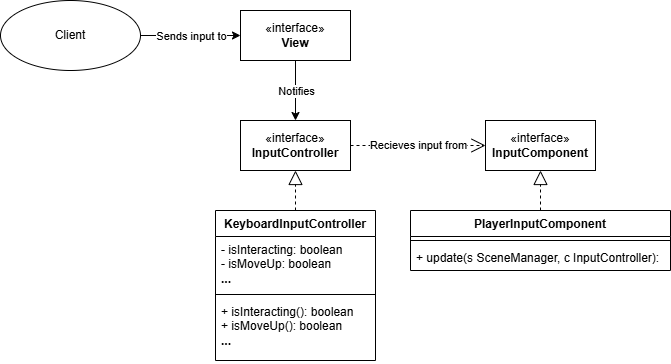
\includegraphics[width=13cm]{ObserverPattern.png}
    \caption{Diagramma UML che rappresenta il flusso degli input.}
    \label{img:ObserverPattern.png}
\end{figure}


\subsection{Ravaioli Alessandro}

\subsection{Tassinari Sabrina}

\subsubsection{Generazione di item in un forziere}

\begin{figure}[H]
    \centering
    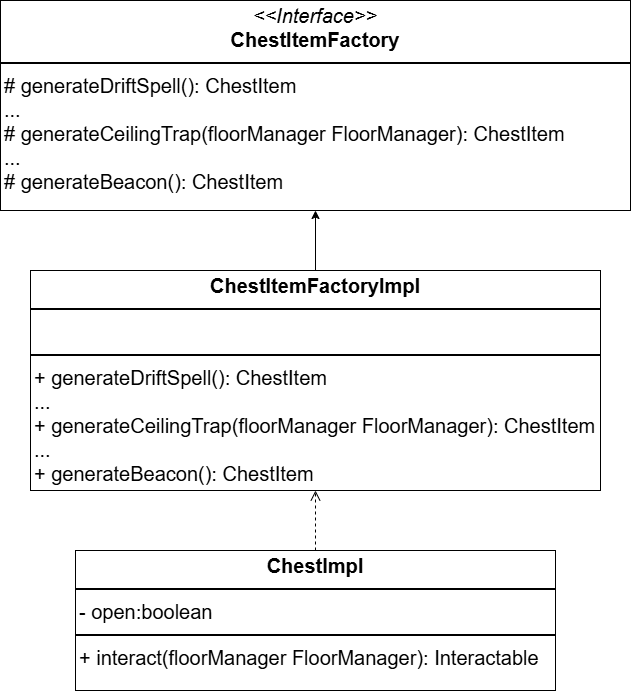
\includegraphics[width=7cm]{patternFactory.drawio.png}
    \caption{Schema UML dell'applicazione del \textit{pattern AbstractFactory} e di dove viene usata la Factory}
    \label{img:chestItemFactory}
\end{figure}

\paragraph{Problema} Il giocatore, esplorando, può trovare dei forzieri, con al loro interno degli items utili oppure delle trappole. 

\paragraph{Soluzione} Per gestire la generazione di item all'apertura della cesta si utilizza il \textit{pattern Abstract Factory}, come da \ref{img:chestItemFactory}.
%
L'interfaccia creatrice fornisce i metodi factory che hanno il compito di creare tutti gli item che si possono trovare nei forzieri, come da \ref{img:chestItemFactory}. 
%
Quando il giocatore interagisce con il forziere utilizzando il metodo \textbf{interact()} viene generato, utilizzando il metodo opportuno, un item scelto in modo randomico tra tutti.

\subsubsection{Riuso del codice per un determinato tipo di item}

\begin{figure}
    \centering
    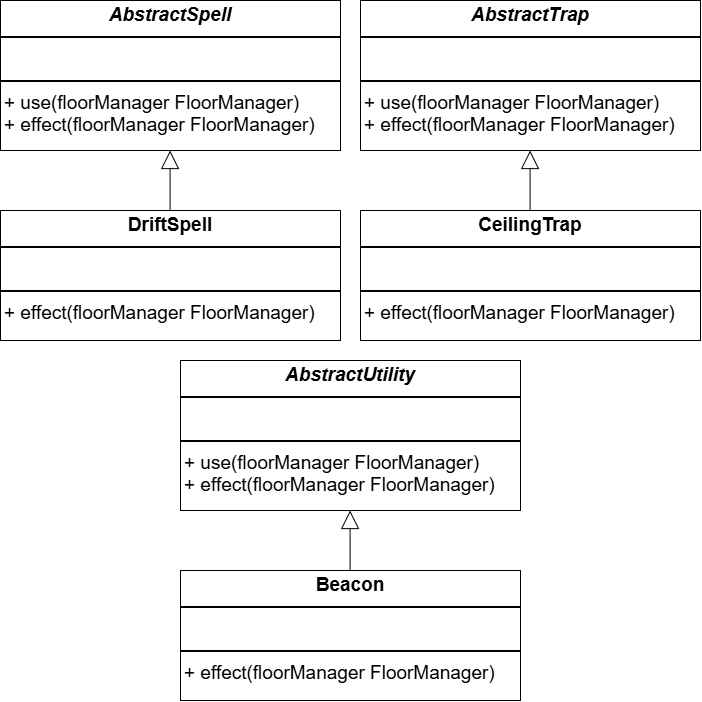
\includegraphics[width=7cm]{patternTemplateItem.drawio.png}
    \caption{Schema UML dell'applicazione del \textit{pattern Template Method}. Si è usato l'esempio del DriftSpell, della CeilingTrap e del Beacon, ma le classi che estendono le classi astratte sono di più.}
    \label{img:templateItem}
\end{figure}

\paragraph{Problema} Sviluppando i vari item che il giocatore può trovare nei forzieri, ci si è accorti che quelli di stesso tipo, quindi incantesimi, trappole e utility, condividono molte caratteristiche.
%
Questo porta a classi molto simili, con metodi ripetuti. 

\paragraph{Soluzione} Ogni tipo di item ha delle caratteristiche simili; è stato quindi utilizzato il \textit{pattern Template Method}, in modo da poter riutilizzare la stessa classe per sviluppare più item, come da \ref{img:templateItem}.
%
Per ogni tipo di item il metodo template è \textbf{use()}, che utilizza il metodo astratto \textbf{effect()}. 

\subsection{Tramonti Daniele}

\subsubsection{Struttura base dei nemici}

\paragraph{Problema} I nemici presenti nel gioco possono essere diversi tra loro, ma presentano tutti la stessa struttura di base che comprende per esempio:

\begin{itemize}
    \item salute
    \item skill
    \item una posizione nella mappa
    \item un livello
    \item un tag che ne identifica il tipo
    \item un campo per definire la visibilità
    \item un campo per definire se il mostro è in un combattimento
\end{itemize}

\paragraph{Soluzione} Ho deciso di utilizzare un un'unica implementazione di una classe astratta \textit{AbstractMonster} che contiene già tutte le caratteristiche di base di un mostro, il quale poi nella sua classe
%
specifica, che estende la classe generale \textit{AbstractMonster}, potrà ricevere qualità personalizzate. La scelta di questa soluzione è stata fatta per permettere:

\begin{itemize}
    \item \textbf{estendibilità:} grazie a questa struttura l'aggiunta di un nuovo mostro è molto semplice;
    \item \textbf{riuso:} con l'utilizzo della classe astratta generale ogni mostro ha la stessa implementazione di base senza però dover duplicare codice per ognuno.
\end{itemize}

\begin{figure}[H]
    \centering
    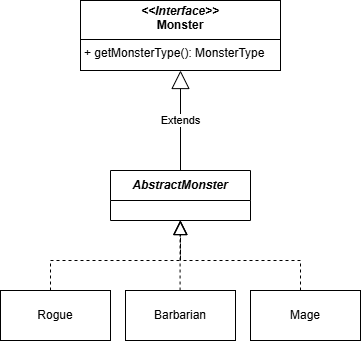
\includegraphics[width=7cm]{AbstractMonster.png}
    \caption{Schema UML dell'uso dell'\textit{Abstract class AbstractMonster}. Si è usato l'esempio del Rogue, del Barbarian e del Mage, ma le classi che la estendono sono di più.}
    \label{img:AbstractMonster}
\end{figure}

\subsubsection{Creazione dei nemici}

\paragraph{Problema} Ogni tipologia di nemico nel gioco ha un preciso piano dove può esistere e compiere azioni, perciò far apparire il mostro corretto nel piano in cui si trova l'avventuriero è
%
tutt'altro che un problema immediato da risolvere.

\paragraph{Soluzione} Per riuscire a trovare una soluzione a questo problema, ho utilizzato il \textit{pattern creazionale Factory Method} per far sì che fosse presente una factory generale
%
con un singolo metodo pubblico da poter essere richiamato. Nella sua implementazione poi sono stati creati dei metodi per generare ogni tipo di mostro che sarebbero stati chiamati, in base
%
al piano in cui il player si sarebbe trovato in quel momento, dal metodo generale. Questa soluzione è stata attuata per:

\begin{itemize}
    \item \textit{facilità nell'uso:} basta richiamare il singolo metodo della factory \textbf{generate()} della factory e genererà in automatico il mostro corretto per quel piano;
    \item \textit{estendibilità:} è possibile aggiungere un metodo specifico nell'implementazione della \textit{factory} per aggiungere un nuovo mostro;
    \item \textit{divisione delle responsabilità:} viene delegato ad una componenente specializzata un compito di cui non si devono interessare altre classi.
\end{itemize}

\begin{figure}[H]
    \centering
    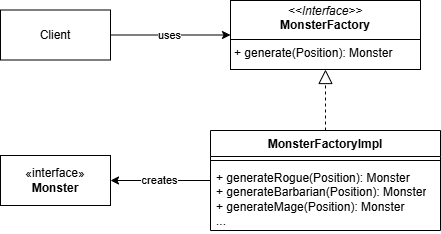
\includegraphics[width=7cm]{FactoryMethod.png}
    \caption{Schema UML dell'applicazione del \textit{pattern creazionale Factory Method}}
\end{figure}

\subsubsection{Movimento dei nemici}

\paragraph{Problema} Ogni nemico si deve muovere nella mappa autonomamente cercando, se possibile, di inseguire ed attaccare l'avventuriero.

\paragraph{Soluzione} Alla fine si è deciso di creare un algoritmo, in modo autonomo, uguale per tutti i mostri con lo scopo di rendere i movimenti il più realistici possibili. Si è fatto 
%
utilizzo di una classe statica separata, denominata \textbf{Ai}, il cui metodo viene chiamato da ogni mostro quando è il proprio turno di muoversi. L'utilizzo di algoritmi come per esempio
%
\textit{Shortest Path di Dijkstra} sono stati scartati per:

\begin{itemize}
    \item \textit{tempistiche:} ricalcolare il percorso migliore per ogni singolo mostro ed ad ogni movimento del player (al massimo circa 10 al secondo) avrebbe potuto portare a tempistiche di calcolo
%
non ottimali e di conseguenza ad un gameplay non performanti.
\end{itemize}

%
La scelta di questa soluzione è stata fatta per permettere:

\begin{itemize}
    \item \textit{facilità nell'uso:} basta richiamare il metodo statico \textbf{move()} della classe \textit{Ai} per ottenere il movimento del mostro;
    \item \textit{divisione delle responsabilità:} viene delegato ad una classe secondaria un compito per non farlo svolgere direttamente alla classe del mostro.
\end{itemize}

\begin{figure}[H]
    \centering
    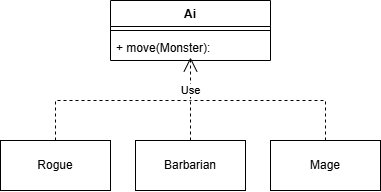
\includegraphics[width=7cm]{MonsterMovement.png}
    \caption{Scherma UML dell'applicazione della \textit{classe statica Ai}. Si è usato l'esempio del Rogue, del Barbarian e del Mage, ma tutte le classi dei mostri fanno riferimento ad \textit{Ai}.}
\end{figure}

\chapter{Sviluppo}

\subsection{Testing automatizzato}
Per testare l'applicazione abbiamo fatto uso di diversi test che testavano i vari elementi del Model:
\begin{itemize}
    \item \textbf{Inventario}, del quale si testa l’inizializzazione e la gestione degli incantesimi.
    \item \textbf{Oro}, del quale si testa: l’inizializzazione, la gestione delle operazioni di acquisizione, perdita e reset dell’oro, il metodo per modificare la capacità massima di oro trasportabile e la meccanica della donazione dell’oro al tempio.
    \item \textbf{Mostri}, dei quali viene testata la generazione idonea nel piano corrispondente, il movimento corretto nelle situazioni in cui si possono trovare e il giusto funzionamento dei danni verso il Player.
    \item \textbf{Player}, del quale si testano una vasta gamma di funzionalità, di seguito illustrate in maggior dettaglio.
\end{itemize} 
%
In merito all'inventario, si verifica che venga inizializzato correttamente con il numero previsto di oggetti, confrontando i valori attesi di pozioni, incantesimi e altri elementi con quelli effettivi. Inoltre, si controlla che 
%
la lista delle mappe dei diversi piani del dungeon non sia nulla. \newline
%
Viene anche effettuato un test sull’incantesimo di invisibilità, utilizzato come campione, per accertarsi che i metodi dedicati alla modifica e alla verifica della sua quantità nell’inventario funzionino correttamente. \newline
%
Relativamente all’oro, si verifica che all’istanziazione il valore iniziale dell’oro corrente sia zero, che la capacità massima di oro trasportabile sia cento e che l’oro donato dal giocatore sia zero. Successivamente, 
%
si controlla che l’oro aggiunto venga accumulato correttamente senza superare la capacità massima. Si testa inoltre che, dopo aver accumulato l’oro, il metodo di reset riporti il valore dell’oro a zero. \newline
%
Viene verificata anche la possibilità di modificare la capacità massima dell’oro, assicurandosi che non si possa superare il limite imposto. Si controlla infine che l’oro donato al tempio possa essere impostato e modificato correttamente,
%
e che la rimozione dell’oro funzioni come previsto, impedendo che il valore dell’oro corrente scenda sotto zero. \newline
%
Per quanto riguarda i mostri si è testato se il loro movimento fosse corretto, se facevano danno al giocatore nei momenti giusti e se i mostri generati in un determinato piano fossero del tipo giusto. \newline
%
Per quanto riguarda il Player, si verifica che venga correttamente inizializzato con i valori di default appropriati e che i metodi setter funzionino correttamente, modificando le sue proprietà.
%
Viene inoltre testata la correttezza dei metodi che incrementano i valori del giocatore, come i punti esperienza ed il numero di nemici uccisi. Si controlla anche che il giocatore possa salire di livello correttamente, 
%
aggiornando i punti esperienza e quelli necessari per il livello successivo. Viene eseguito un test per verificare che il giocatore possa muoversi correttamente, aggiornando la sua posizione nel piano. \newline
%
Per quanto riguarda le battaglie, i test sono suddivisi in due scenari: se il giocatore vince lo scontro, si verifica che ottenga le ricompense previste, come i punti esperienza e l’aumento del contatore dei nemici uccisi;
%
se il giocatore perdem si verifica che venga dichiarato morto e che non possa più combattere. Inoltre, si controlla che il giocatore infligga danni correttamente al mostro e che riceva danni in risposta. Si verifica anche 
%
che il giocatore venga dichiarato morto alle condizioni appropriate. \newline
%
Vengono eseguiti due test sulla rigenerazione: uno per verificare che avvenga dopo un certo periodo di tempo in condizioni normali, uno per confermare che avvenga in un quinto del tempo quando l’incantesimo di rigenerazione 
%
è attivo e il giocatore si trova in un tempio. \newline
%
Infine, si verifica che l’utilizzo degli oggetti dell’inventario riduca correttamente la quantità disponibile e che la profondità massima raggiunta dal giocatore nel dungeon venga aggiornata correttamente. \newline
%
Per quanto riguarda gli items si è testato se la loro generazione fosse corretta e se il loro funzionamento era giusto, quindi se quando venivano usati il loro numero decrementava e se quando venivano trovati il loro numero aumentava. \newline
%

\subsection{Note di sviluppo}

\subsubsection{Bulgarelli Marco}

\subsubsection{Ravaioli Alessandro}

\subsubsection{Tassinari Sabrina}
\paragraph{Utilizzo di lamba expression}
Utilizzate in: "INSERIRE PERMANENT LINK ALLA RIGA DOVE SI UTILIZZA"

\paragraph{Utilizzo di Stream}
Utilizzati in: "INSERIRE PERMANENT LINK ALLA RIGA DOVE SI UTILIZZA"

\paragraph{Utilizzo di Optional}
Utilizzati in: "INSERIRE PERMANENT LINK ALLA RIGA DOVE SI UTILIZZA"

\subsubsection{Tramonti Daniele}
\paragraph{Utilizzo di Stream e lambda expression}
Esempio di codice dove vengono utilizzati entrambi:
\begin{sloppypar}
\url{https://github.com/ravag/OOP24-fargoal/blob/cb5f09a083bb0696ec37722b48ac348cbd7187d8/src/main/java/fargoal/model/entity/monsters/ai/Ai.java#L109C9-L120C18}
\end{sloppypar}

\chapter{Commenti finali}

\subsection{Autovalutazione e lavori futuri}

\subsubsection{Bulgarelli Marco}

\subsubsection{Ravaioli Alessandro}

\subsubsection{Tassinari Sabrina}
Per quanto riguarda la mia parte del lavoro, mi sono occupata degli Interectable, quindi degli oggetti magici con cui il giocatore interagisce nel gioco.
%
Sono rimasta soddisfatta del mio lavoro e di quello dei miei compagni: siamo riusciti ad implementare le funzioni obbligatorie che ci eravamo posti inizialmente e fra di noi abbiamo lavorato bene. 
%
Inoltre, questo progetto mi ha aiutato molto per quanto riguarda la crescità delle mie abilità: precedentemente non mi ero mai cimentata in un progetto di questo tipo e penso di aver imparato molto nell'ambito della programmazione e del lavoro in gruppo.
%
In futuro mi piacerebbe ritornare su questo progetto aggiungendo nuovi oggetti magici e questo mi sarà facile farlo, grazie al modo in cui ho implementato le classi.
%
 

\subsubsection{Tramonti Daniele}
Io nel progetto ho avuto il compito di creare i mostri e di prendermi cura del loro movimento.
%
Questa esperienza, anche se certe volte un po' faticosa, è stata però un bel momento di crescita personale e tecnica verso la programmazione con Java, ma soprattutto è stata un'occasione
%
ottima per sperimentare il lavoro in team, che penso sia una delle principali challenge nell'ambiente lavorativo della programmazione. Sono anche abbastanza soddisfatto del risultato che 
%
rispecchia molto l'idea che ci eravamo posti all'inizio e rimane abbastanza fedele al gioco originale al quale ci siamo ispirati. Sicuramente, se in futuro avrò tempo e occasione, non mi tirerò
%
indietro dall'ottimizzare lo sviluppo del gioco e migliorarlo negli aspetti che troveremo interessanti da aggiungere. Infine sono rimasto molto contento anche del corso di OOP, un corso molto
%
interessante e che, seppur partendo da zero con la programmazione in Java, è stato in grado di accompagnarmi molto bene nell'apprendimento di questo nuovo linguaggio, merito soprattutto ai docenti
%
che sono stati sempre molto professionali, chiari e disponibili per ogni richiesta.


\subsection{Difficoltà incontrate e commenti per i docenti}

\appendix
\chapter{Guida utente}

Il giocatore, quando aprirà l’applicazione si troverà di fronte la schermata iniziale del gioco. 
%
Si potrà scegliere, premendo la \underline{barra spaziatrice}, tra due opzioni: \textbf{START GAME} oppure \textbf{EXIT}.
%
Per poter iniziare a giocare si scelga con le \underline{frecce ↑ e ↓}  la scritta \textbf{START GAME}, colorandola di \textit{azzurro}, in questo modo si potrà iniziare a giocare.
%
Quando la partità inizia il giocatore si troverà nella mappa del primo livello del dungeon.
%
Noterà che essa sarà quasi tutta oscurata, tranne la parte dove l’avventuriero si trova. 
%
Esso, muovendosi, potrà scoprire altre zone della mappa, che diventerà visibile mano a mano che si esplora il piano.
%
Per muovere l’avventuriero si dovranno premere le frecce ← per andare a sinistra, ↑ per andare verso l’alto, → per andare a destra e ↓ per andare verso il basso.
%
Per \textbf{ingaggiare un combattimento} con i mostri presenti nel piano basterà solo \underline{avvicinarsi} e il combattimento inizierà da solo.
%
Nel piano, inoltre, ci saranno degli oggetti con i quali il giocatore potrà interagire.
%
Per interagire con il \textbf{tempio} il giocatore dovrà solo \underline{posizionarsi sopra quello}, in automatico i soldi verranno donati e il giocatore sarà immune a qualsiasi attacco.
%
Per interagire con altri oggetti, quali \textbf{scale per scendere e salire in piani differenti}, \textbf{sacche di monete} e \textbf{ceste} va invece premuta la \underline{barra spaziatrice}.
%
In particolare i sacchi di monete potrebbero contenere più monete di quelle che si possono portare: i soldi in più verranno sotterrati nel punto dove la sacca d’oro è stata trovata, in attesa che il giocatore abbia abbastanza spazio nell’inventario per riprendere le monete premendo di nuovo la \underline{barra spaziatrice}. 
%
\\
%
Nelle ceste, oltre a trappole che danneggiano il giocatore, verranno trovati degli oggetti che saranno aggiunti direttamente nell’inventario.
%
Gli oggetti in questione sono:
%
\begin{itemize}
    \item \textbf{Drift spell}: questo incantesimo viene usato premendo il \underline{tasto D}. Esso, se attivo, non fa danneggiare il giocatore quando cade in un buco. Quando l'avventuriero apre una cesta, infatti, potrebbe trovare una trappola di nome \textit{pit}, che può essere evitata lanciando questo incantesimo.
    \item \textbf{Invisibility spell}: questo incantesimo viene usato premendo il \underline{tasto I}. Esso rende invisibile il giocatore ai mostri. 
    \item \textbf{Light spell}: questo incantesimo viene usato premendo il \underline{tasto L}. Esso permette di espandere l’area illuminata della mappa. Il giocatore, quindi, scopre aree maggiori andando avanti nella mappa. Quando l’incantesimo è attivato, però, se l’incantesimo dell'invisibilità è attivo il giocatore è visibile ai mostri. Si può accendere o spegnere la luce premendo il tasto O.
    \item \textbf{Regeneration spell}: questo incantesimo viene usato premendo il \underline{tasto R}. Esso rende la rigenerazione della salute dell’avventuriero il doppio più veloce; viene quindi riacquistato un punto ferita ogni 5 secondi; normalmente, infatti, verrebbe riacquisito un punto ferita ogni 10.
    \item \textbf{Shield spell}: questo incantesimo viene usato premendo il \underline{tasto S}. Esso rende invulnerabile il giocatore nello scontro successivo.
    \item \textbf{Teleport spell}: questo incantesimo viene usato cliccando il \underline{tasto T}. Il giocatore viene teletrasportato vicino ad una torcia, cioè un \textit{beacon}, se posizionato precedentemente dal giocatore nella mappa, o in una posizione casuale.
    \item \textbf{Beacon}: questo oggetto viene posizionato a terra premendo il \underline{tasto B}. Quando esso è a terra il giocatore, se vicino ad esso, è invulnerabile.
    \item \textbf{Enchanted weapon}: questo oggetto incrementa la skill del giocatore, incrementa quindi il danno che il giocatore fa in combattimento.
    \item \textbf{Healing potion}: premendo il \underline{tasto H} il giocatore può bere una pozione di cura, che farà recuperare all’avventuriero dei punti ferita. Essa viene bevuta in automatico, a patto che l'avventuriero ne abbia una in inventario, se il giocatore ha tra i -5 e i 0 punti ferita.
    \item \textbf{Magic sack}: sono delle sacche nelle quali viene posizionato l’oro che il giocatore trova nel dungeon. Ogni sacca può contenere 100 monete e l’avventuriero, inizialmente, ha solamente una di queste nell’inventario.
    \item \textbf{Map}: il giocatore potrà trovare delle mappe di determinati livelli del dungeon; quando il giocatore arriverà a quel piano la mappa sarà illuminata, non buia.
\end{itemize}
%
Per quanto riguarda gli oggetti che si possono utilizzare premendo un tasto, se non si ha il tipo di oggetto del quale si preme il tasto non succede nulla.
%
\\
%
Il gioco procede fino a che il giocatore non finisce i suoi punti vita (quindi arriva a -5) oppure fino a che non ritorna in superficie con la leggendaria Spada di Fargoal, che appare tra il quindicesimo e il ventesimo piano del dungeon e può essere raccolta premendo la \underline{barra spaziatrice}.
%
Quando il gioco finisce comparirà la schermata di fine partita, dalla quale il giocatore potrà scegliere, sempre con le frecce, se giocare una nuova partita o uscire dall'applicazione.

\end{document}